\documentclass{beamer}
\usepackage[utf8]{inputenc}
\usepackage{graphicx}

\hypersetup{
    colorlinks,%
    citecolor=blue,%
    filecolor=blue,%
    linkcolor=blue,%
    urlcolor=blue 
    %urlcolor=mygreylink     % can put red here to better visualize the links
}

\author[Sowmya Vajjala]{Instructor: Sowmya Vajjala}

\title[LING 520]{LING 520: Computational Analysis of English}
\subtitle{Semester: FALL '16}

\date{15 November 2016}

\institute{Iowa State University, USA}
%%%%%%%%%%%%%%%%%%%%%%%%%%%

\begin{document}

\begin{frame}\titlepage
\end{frame}

\begin{frame}
\frametitle{Class Outline}
\begin{itemize}
\item NLP Applications: Information Extraction and Machine Translation %20min - asking questions on what may one need for each app.
\item Information Extraction %15 min
\item Machine Translation %15 min (additionally: 15 + 15)
\item Reminder: Assignment 5 submission due - tonight.
\end{itemize}
\end{frame}

\begin{frame}
\frametitle{Regarding Assignment 5 - Question 1}
\begin{itemize}
\item If you started working on A5 in the past 1-2 days, you may have noticed something is wrong with Stanford Parser online demo.
\item Here are three options to answer Question 1 in this case:
\begin{enumerate}
\item Use any other parser demo online and do the question 1
\item use Stanford parser GUI that comes with the download (refer to README to know how)
\item Write python code to print Stanford parser outputs and analyse that. (which you perhaps did in question 3)
\end{enumerate}
\end{itemize}
\end{frame}

\begin{frame}
\frametitle{NLP applications - overview}
\begin{itemize}
\item \textit{Text classification} - we discussed a few weeks back.
\item \textit{Information extraction}
\item \textit{Machine Translation}
\item Information retrieval (Search)
\item Dialog systems/conversational agents
\item Question Answering/Summarization
\end{itemize}
\end{frame}
%All models are wrong; some models are useful".

\begin{frame}
\frametitle{}
\Large Information Extraction
\end{frame}

\begin{frame}
\frametitle{Information Extraction - overview}
\begin{itemize}
\item Task: Extract different types of information (names, dates, relationships etc) from text.
\item Let us take an example text:
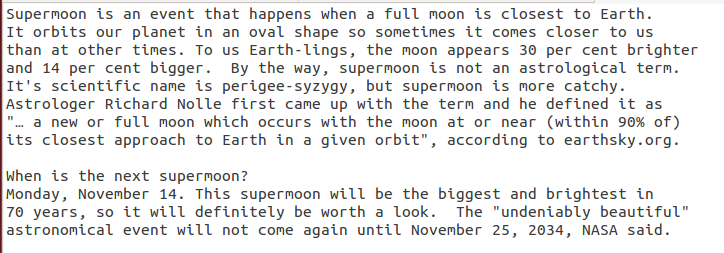
\includegraphics[width=\textwidth]{supermoon.png}
\end{itemize}
\end{frame}

\begin{frame}
\frametitle{Information Extraction - tasks}
\begin{itemize}
\item identify and classify "named entities" in the text - Named Entity Recognition (Supermoon, perigee-syzygy, Richard Nolle, NASA)
\item Not sufficient to just say something is a proper noun. What sort of proper noun is it? person, event? organization? place? \pause
\item Event detection. Key events in our example: supermoon, its next occurrence, etc. \pause
\item Temporal Expressions: Monday, November 14, November 25, 2034 etc. \pause
\item All this information is useful for: Relation extraction (identifying that Richard Nolle is the scientist who coined the term Supermoon)
\end{itemize}
\end{frame}

\begin{frame}
\frametitle{Information Extraction - Methods}
\begin{itemize}
\item Regular expressions (If you know the patterns of named entities, temporal expressions etc)
\item Machine learning (If we do not know the patterns)
\item Example: NER can be seen as a sequence labeling problem like in POS tagging, coupled with gazetteers containing names of persons, organizations etc.
\end{itemize}
\end{frame}

\begin{frame}
\frametitle{Information Extraction and NLTK}
\begin{itemize}
\item NER example (NER.py)
\item Relation extraction example (RelExtraction.py)
\end{itemize}
\end{frame}

\begin{frame}
\frametitle{Some current IE projects: code and data}
\begin{itemize}
\item openIE - \url{http://knowitall.github.io/openie/}
\item reVerb project - \url{http://reverb.cs.washington.edu/}
\item Google relation extraction corpus \\  \url{https://research.googleblog.com/2013/04/50000-lessons-on-how-to-read-relation.html}
\end{itemize}
\end{frame}

\begin{frame}
\frametitle{}
\Large Machine Translation
\end{frame}

%One example slide 

\begin{frame}
\frametitle{Machine Translation}
\begin{itemize}
\item Task: translate text from one language to another (text can be a word, a sentence, a paragraph, a full document)
\item Primary issues in solving the task:
\begin{enumerate}
\item Different scripts, different word orders, different orthographic rules (no caps, no punctuation etc), different morphological structure \pause
\item Understanding genre specific nuances (translating news versus translating a novel)
\item advanced issues: stylistic and cultural differences, idioms, metaphors etc. \pause
\item degrees of automatic translation: rough translation, translation + post editing, high-quality translation for very targeted domain specific language.
\end{enumerate}
\end{itemize}
\end{frame}

\begin{frame}
\frametitle{Machine Translation - Usage scenarios}
\begin{itemize}
\item Rough translation: translating webpages for a general purpose reader
\item Translation with post-editing: translation of software manuals for localization (Computer aided human translation). Computer does some part of translation followed by human translator edits.
\item domain specific: weather forecasts (where vocabulary is limited, and language patterns are also limited).
\end{itemize}
\end{frame}

\begin{frame}
\frametitle{Machine Translation - Classical view}
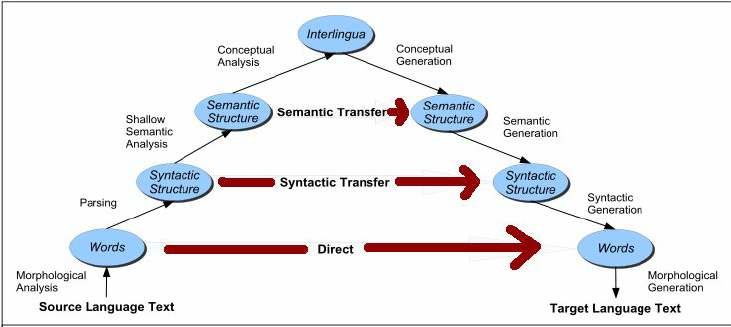
\includegraphics[width=\textwidth]{interlingua.png}
\\ source: \url{https://goo.gl/slXqkS}
\end{frame} %Vauquois triangle

\begin{frame}
\frametitle{Rule based MT}
\begin{itemize}
\item Direct translation: do direct word by word translation from source to target. Not used now, but the same intuition of incremental translation works in currently used systems too.
\item Transfer rules based translation: have rules for translating form X to Y, to account for word-order differences, and other such issues in addition to lexical transfer rules.
\item Direct + transfer rules based translation
\end{itemize}
\end{frame} %PBMT

\begin{frame}
\frametitle{Machine Translation - Statistical view}
\framesubtitle{Bayes is Back!}
\begin{itemize}
\item Idea: If you have a large collection of parallel sentences from source and target languages, you can approximate human translation with a statistical model.
\item If F is a foreign language and we are translating from F to English, probability of best translation:
\\ = argmax$_{E \in English }$ P(F$|$E)*P(E)
\item Where P(E) is the language model for target language (English), which helps us choose the translation that is most likely in English language
\item P(F$|$E) is the translation model. A commonly used translation model is "Phrase Based Statistical Machine Translation".
\item Challenge: Creating alignments between the source and target sentences in the training data. 
\end{itemize}
\end{frame} %PBMT

\begin{frame}
\frametitle{Machine Translation - Statistical view}
\framesubtitle{An example phrase table. source: \url{https://goo.gl/cORL3E}}
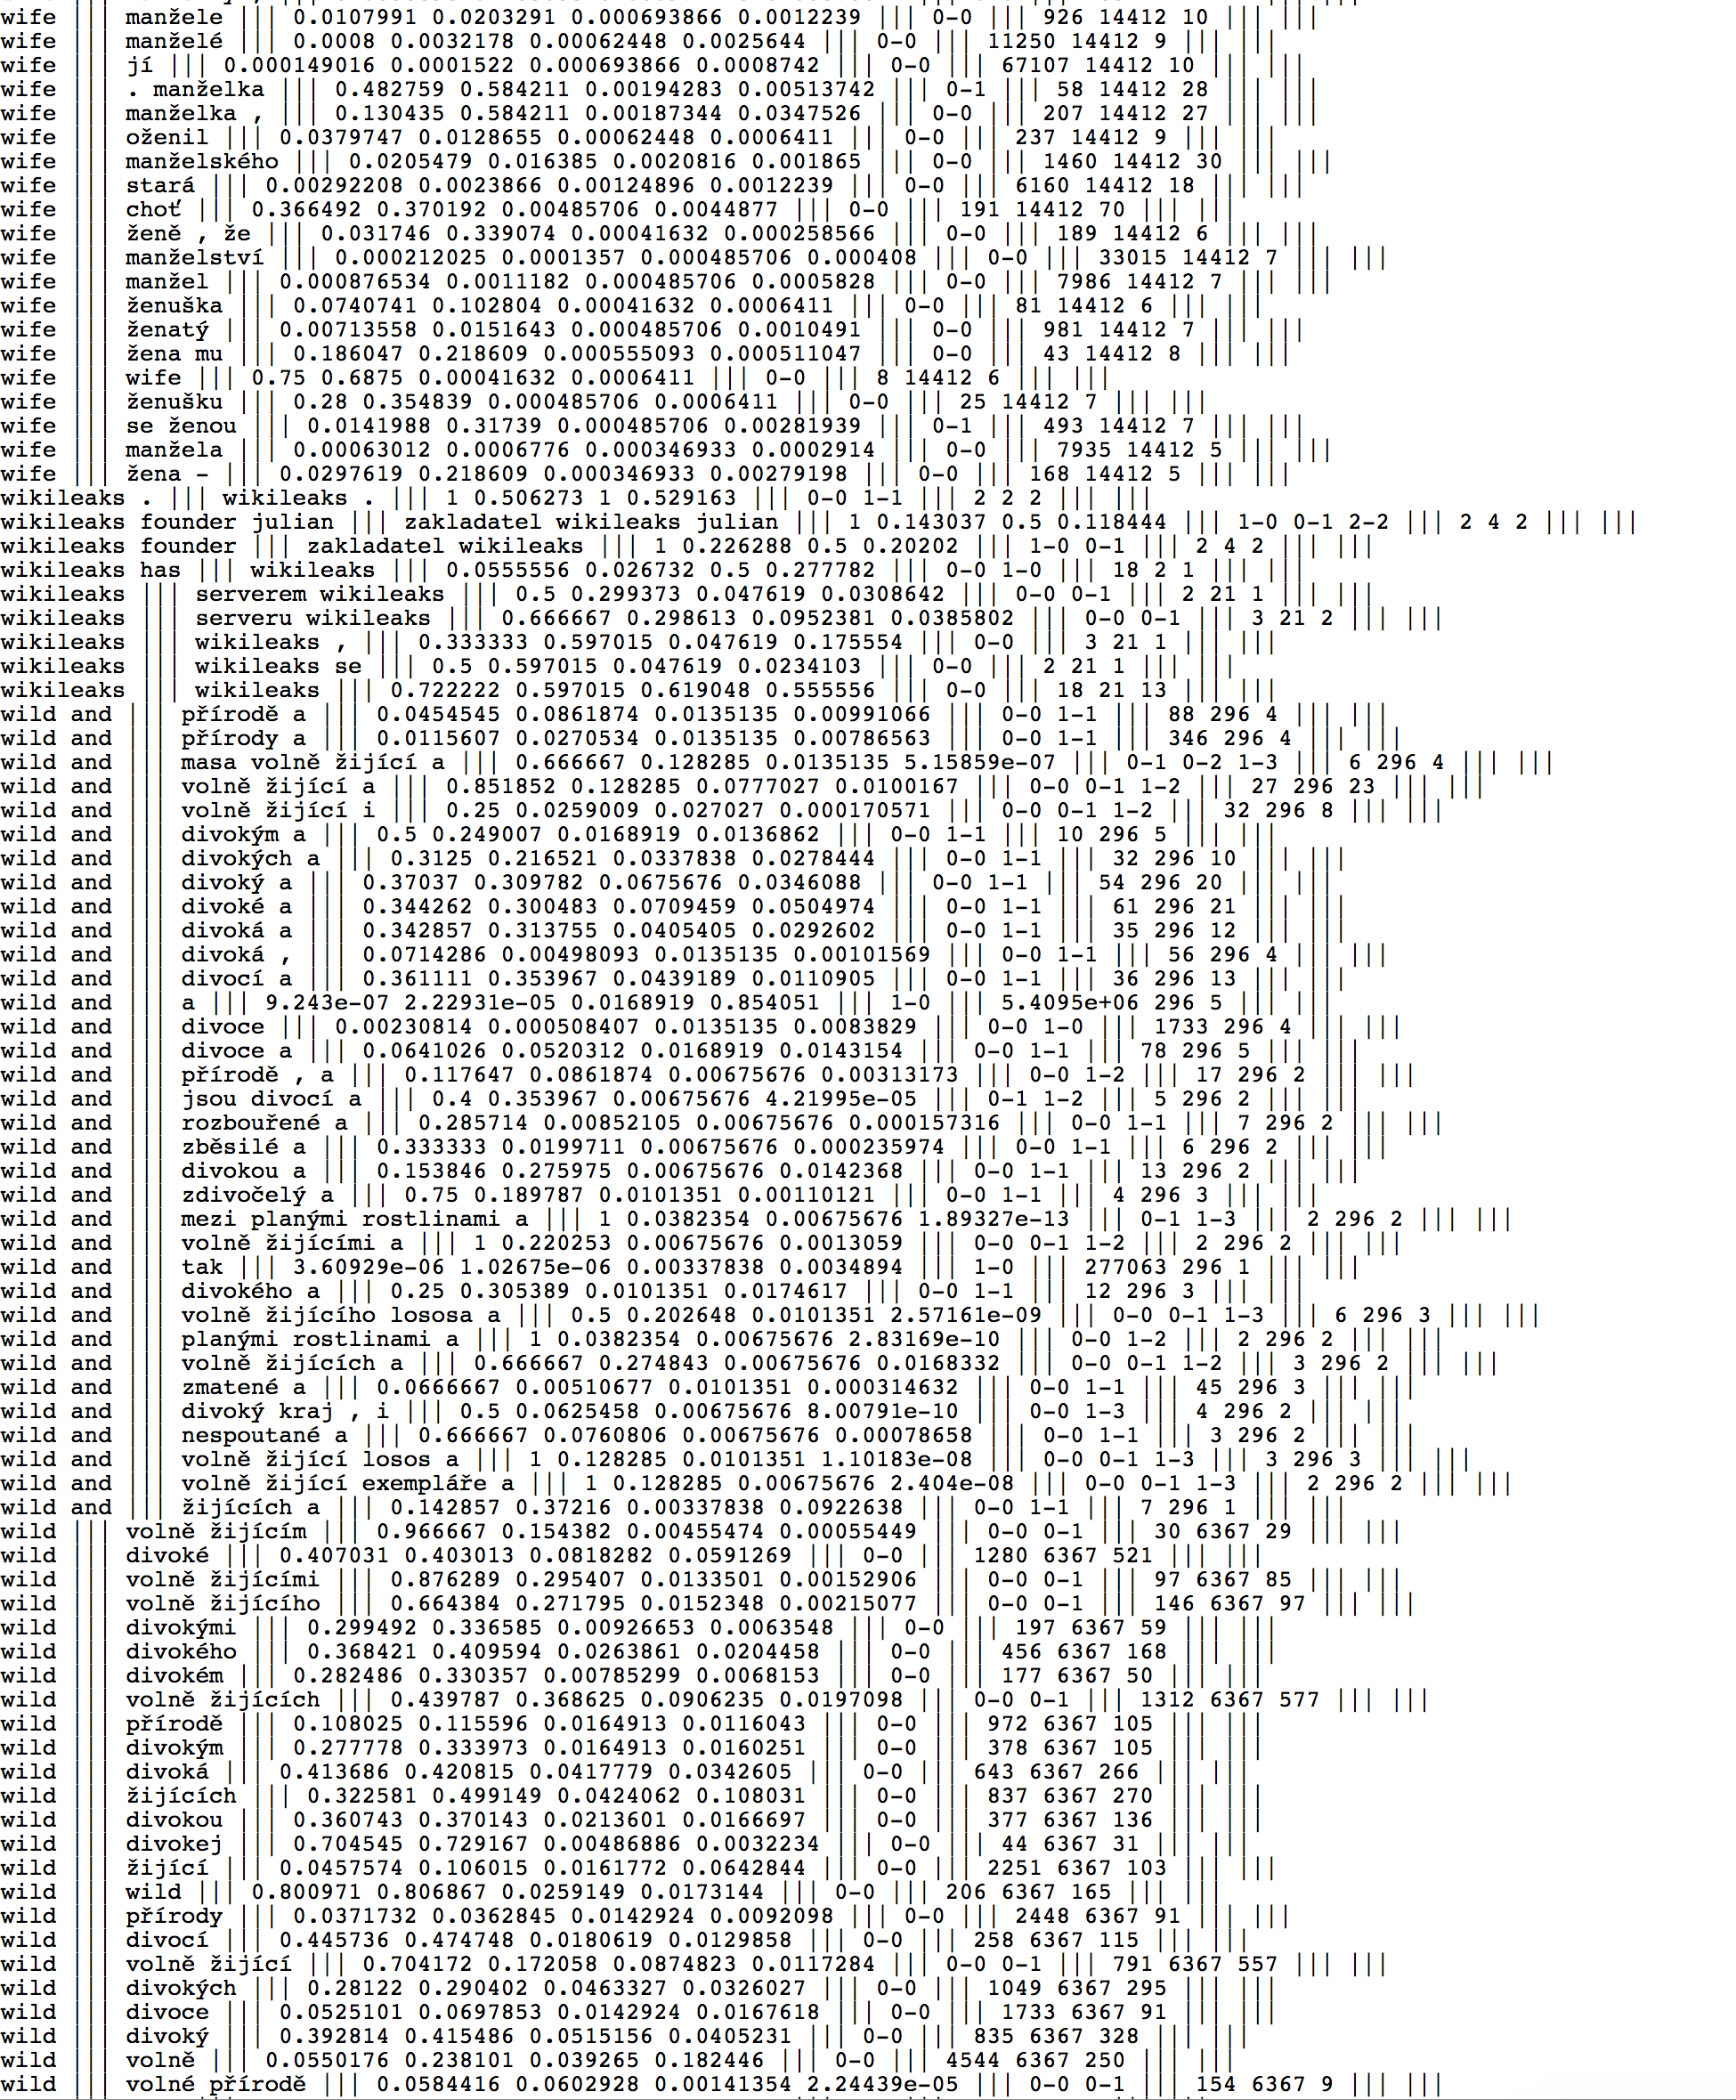
\includegraphics[width=0.6\textwidth]{PhraseTable.png}
\end{frame} %PBMT

\begin{frame}
\frametitle{Evaluating MT systems}
\begin{itemize}
\item Human raters (in terms of: correctness, clarity, naturalness, grammaticality etc)
\item automatic evaluation - BLEU score (ngram similarity based measure between a translated sentence and a gold standard human translation)
\item Other automatic measures: TER, METEOR, NIST etc. 
\end{itemize}
\end{frame} %PBMT

\begin{frame}
\frametitle{Useful Resources}
\begin{itemize}
\item Chapter 25 in Jurafsky and Martin (very comprehensive overview)
\item \url{http://www.statmt.org/} - comprehensive website on readings, software, corpora related to developing and testing statistical machine translation systems.
\item \url{https://www.apertium.org} - open source machine translation platform that lets you create rule-based MT models.
\item Google Translate, Bing Translate etc - MT applications in real life.
\end{itemize}
\end{frame}

\begin{frame}
\frametitle{Exercise in Analyzing machine translation}
\begin{itemize}
\item Two popular machine translation software online: Google Translate and Bing translate
\item Task: Try out how both these tools work for translating from English to your native language and viceversa (Native English speakers: choose another language you know. If you know only English, pair up with some other person).
\item Spend some time with these and we can discuss your observations towards the end of the class.
\end{itemize}
\end{frame}

\begin{frame}
\frametitle{Next class}
\begin{itemize}
\item NLP for CALL - Introduction
\item Assignment 5 discussion
\item Final projects - status and discussion 
\item Recommended Readings: Burstein (2009), Chapelle and Chung (2010). Meurers (2013). Read atleast two of them. Large amount of thursday's class invovles discussion about these papers. 
\item Optional readings: Chapters on Writing Aids and Tutoring Systems in Language and Computers.
\end{itemize}
\end{frame}


\end{document}

\begin{frame}
\frametitle{Programming exercise - 1}
\begin{itemize}
\item Take any .txt version file from gutenberg.org, written by your favorite author (in English!)
\item Read that file into your python code, and do the following using NLTK:
\begin{enumerate}
\item Split the file into sentences.
\item Print the following: number of sentences in the file, average sentence length (in number of words), average word length (in number of characters), number of unique words, number of unique stems.
\item Note 1: Once sentence splitting is done, you can ignore punctuation markers for the rest of the calculation.
\item Note 2: You can use any stemmer you want.
\end{enumerate}
\end{itemize}
\end{frame}

\begin{frame}
\frametitle{Programming exercise - 1}
\begin{itemize}
\item For the same file from last slide, do the following:
\item Read that file into your python code, and do the following using NLTK:
\begin{enumerate}
\item Split the file into sentences.
\item For each sentence, print its POS tagged version as a string of tags. E.g., if you have "It is a sentence" as your sentence, and your NLTK tagger outputs the tags for this sentence as a list (or tuple or whatever), you should print the tag as a string. E.g., PRP VBZ DT NN (not as [PRP, VBZ, DT, NN] or as [(It, PRP), (is, VBZ) .. ... ])
\end{enumerate}
\end{itemize}
\end{frame}
